% Chapter 1

\chapter{Mixed-species aggregation in arthropods - a review} % Main chapter title

\label{Chapter1} % For referencing the chapter elsewhere, use \ref{Chapter1} 

\lhead{Chapitre 1. \emph{Mixed-species aggregation in arthropods - a review}} % This is for the header on each page - perhaps a shortened title

Julien \textsc{Boulay}\up{a,b}, Valéry \textsc{Hédouin}\up{a} and Damien \textsc{Charabidzé}\up{a}

\up{a} Univ. Lille, CHU Lille, EA 7367 - UTML - Unité de Taphonomie Médico-Légale, Lille, France\\
\up{b} Université Libre de Bruxelles, Unit of Social Ecology, Brussels, Belgium\\


Article soumis à \emph{Behavioral Ecology}.


\cleardoublepage

%----------------------------------------------------------------------------------------
%	SECTION 1
%----------------------------------------------------------------------------------------
	\section{Lay summary}
Mixed-species groups are found in a large range of taxa. We reviewed the original research on mixed-species groups and collective behavior in arthropods and highlight the tools that have been used to study and quantify this type of aggregation. The existence of such groups raises questions about the evolution of sociality in animals and the mechanisms involved in cross-species recognition. Finally, this review questions how individuals aggregate with closely related species and the benefits of such groupings. 

	\section{Abstract}
In nature, mixed-species groups are commonly found in mammals and birds, and they have been studied in a collective behavior context. Such mixed-species groups are also observed in a large range of arthropod taxa independent of their level of sociality. Here, we offer the first synthesis of the research on mixed-species groupings in arthropods and highlight the behavioral and evolutionary questions raised by such behavior. As non-mixed (monospecific) groupings provide benefits to individuals, the advantages offered by groupings are described and discussed. These advantages can be attributed to the increase in group size and could be considered to be identical to those of non-mixed groupings (e.g., protection against predators). Furthermore, the competition-cooperation phenomena that might be involved between the species in a group are examined as are the metrics and models commonly used to study heterospecific groups of animals. Several examples are presented to highlight the mechanisms underlying such groupings, particularly the evidence for phylogenetic proximity between members. The study of mixed-species groups offers biologists an interesting way to explore the frontiers of cooperation-competition, especially the process of sympatric speciation.

\textit{Keywords}: complex system, collective behavior, cross-species recognition, self-organization, sociality.

\clearpage

%----------------------------------------------------------------------------------------
%	SECTION 2
%----------------------------------------------------------------------------------------
	\section{Background}
Over the last 40 years, the research on collective behavior has rapidly expanded. In a milestone book entitled \textit{Living in Groups}, Krause and Ruxton \cite{krause_living_2002} reviewed the concepts underlying group living. They focused their work on the mechanisms that govern the evolution and maintenance of animal groups in several species. In 2010, \citet{sumpter_collective_2009} reviewed how the mechanisms driving group behavior are intertwined with understanding its functions; indeed, simple rules may generate very impressive and complex systems, such as migrating flocks of starlings, schools of fish or wildebeest herds. In this context, the idea of self-organization has been increasingly applied to the study of collective phenomena. Self-organization successfully explains how simple interactions between individuals can generate complex collective systems. Furthermore, self-organization is always associated with the notion of emergence; a phenomenon is emergent when observers cannot predict its appearance based only on the knowledge of the behavior of components' system to which it belongs. More poetically, self-organization is \textit{a mess organizer} for Edgar Morin \cite{morin_methode_1977}. From unicellular organisms to mammals, this theory has been used to describe collective phenomena and to explain how individuals can form, amplify, regulate or divide groups, and many examples of emergent phenomena are described in \citet{camazine_self-organization_2001}. However, most authors have only focused on monospecific groups \citep{stamps_conspecific_1988,camazine_self-organization_2001,sumpter_collective_2009,kivela_past_2014}.

Intraspecific collective behavior is actually poorly understood and has essentially only been studied in arthropods (see the review by \citet{jeanson_key_2012}), although some studies of heterospecific groups of mammals or birds can be found in the literature \citep{terborgh_mixed_1990,stensland_mixed_2003}. In fact, a large majority of the publications are focused on eusocial species, especially ants and bees \citep{wilson_insect_1971,krause_living_2002,sumpter_collective_2009}, which is especially surprising considering the small number of eusocial insect species. Of 900 000 known insect species, eusocial insects represent only 2$\%$ but are the topic of 78$\%$ of the scientific publications related to insects \citep{costa_social_2005,wilson_eusociality:_2005}. A common example of a mixed colony involves a \textit{Temnothorax americanus} (the acorn slave-raiding ant) parasitic queen invading a \textit{T. curvispinosus} nest to take the place of the legitimate queen and use her workers to rear the \textit{T. americanus} offspring. During this process, both species can be found working and living together in the nest, but after some time, all of the host workers die leaving only the parasitic ants to occupy the nest. This temporary association challenges the conventional definition of an interspecific aggregation and highlights the unstable balance between different species that share the same ecological niche. True interspecific aggregations can actually be found in species with low levels of sociality (e.g., gregarious or communal; see the classification of sociality in \citet{wilson_insect_1971}). A few interspecific associations have also been reported to arise from in vitro interspecific breeding \citep{fielde_artificial_1903,errard_development_1994,vauchot_regulation_1996} (Table \ref{tab:mixedsp}).

This review attempts to assemble a comprehensive inventory of mixed-species arthropod groups through the perspective of collective behavior. We redefine the common notion of gregariousness as it applies to multi-species groups, and we examine the benefits offered by such aggregations in comparison to those gained from non-mixed groups. Then, we examine the frontier between cooperation and competition in the context of collective behavior and discuss the mechanisms underlying mixed-species groups based on the evidence for phylogenetic proximity among member species, which permits cross-species recognition. Finally, we propose future research that will provide biologists with an interesting way to explore the evolution of mixed-species groups.


%----------------------------------------------------------------------------------------
%	SECTION 3
%----------------------------------------------------------------------------------------
	\section{Definition}
Several terms are used in the literature for groups composed of individuals of different species, including mixed-species, multi-species, interspecific, heterospecific or polyspecific. For the sake of clarity, the term mixed-species will be used throughout this review, and it can refer to closely related species, species from different taxa or species from different orders \cite{stensland_mixed_2003}. Two distinct notions can be used to characterize animal species that form groups: gregariousness and social-tolerance.

If characterized by the underlying mechanisms, gregariousness is an active behavior, whereas tolerance is passive. Indeed, \textit{'a species' social tolerance (that) has evolved to fit its optimal population density and optimal population structure} \cite{barrows_animal_2011}, and this definition implies that individuals do not recognize or use aggregation vectors. In contrast, gregariousness is defined by \citet{vulinec_collective_1990} as \textit{the tendency of an animal to aggregate with others such that the animals are in contact with one another, or are nearly so, and that the distribution of the animals in the local environment is extremely patchy.} When considering this definition, it is also important to include the idea of inter-attraction, which permits animals to create such groups. In other words, individuals must have a way to share information between group members. It is also important to separate temporary groupings of individuals (groups that only form for mating or are created by environmental stimuli) from gregariousness. This review focuses on mixed-species aggregations, i.e., groups where members of different species actively aggregate and remain together regardless of environmental heterogeneity or reproductive attraction (Figure \ref{fig:agregmix}).

The notion of gregariousness often implies cooperation and/or competition, and these two phenomena are the most fundamental principles that drive the evolution of social structures. In 1931, Warder C. Allee \cite{allee_animal_1931} was the first to observe and to experimentally test for a positive relationship between a fitness component and population size or density \citep{stephens_consequences_1999,courchamp_allee_2008}. Based on this pioneering study, \citet{odum_fundamentals_1953} named this idea \textit{the Allee principle}, which is more widely known as the ‘Allee effect’, which mainly impacts survival and reproduction. Indeed, aggregation offers direct benefits for group members and gathers reproductive individuals together, thereby facilitating reproduction. However, there are only a few empirical and theoretical studies of the consequences of the Allee effect for mixed-species animals groups \cite{courchamp_inverse_1999}. In one of the few known cases, Kyogoku and Nishida \cite{kyogoku_presence_2012} observed an Allee effect in female beetles due to the presence of males from a different species because \textit{Callosobruchus maculatus} females are able to mate with both \textit{C. maculatus} and \textit{C. chinensis} males. Accordingly, the presence of both species offers \textit{C. maculatus} females more reproductive partners, thus increasing the probability of reproductive success \cite{kyogoku_presence_2012}. Interestingly, this is not a two-way reproductive relationship as \textit{C. chinensis} females are not able to mate with \textit{C. maculatus} males. Such interesting observations challenge the common definition of a \textit{species} as \textit{related individuals that resemble one another, are able to breed among themselves, but are not able to breed with members of another species} (Random House Webster’s Dictionary). Moreover, the definition of aggregation is also complicated as the gathering of these two species is mediated by reproduction, which contradicts the definition presented above. Based on this example, the study of mixed-species groups offers biologists an interesting way to explore the frontiers of such concepts, especially the sympatric speciation process. 


 \begin{figure}[ht]
	\centering
		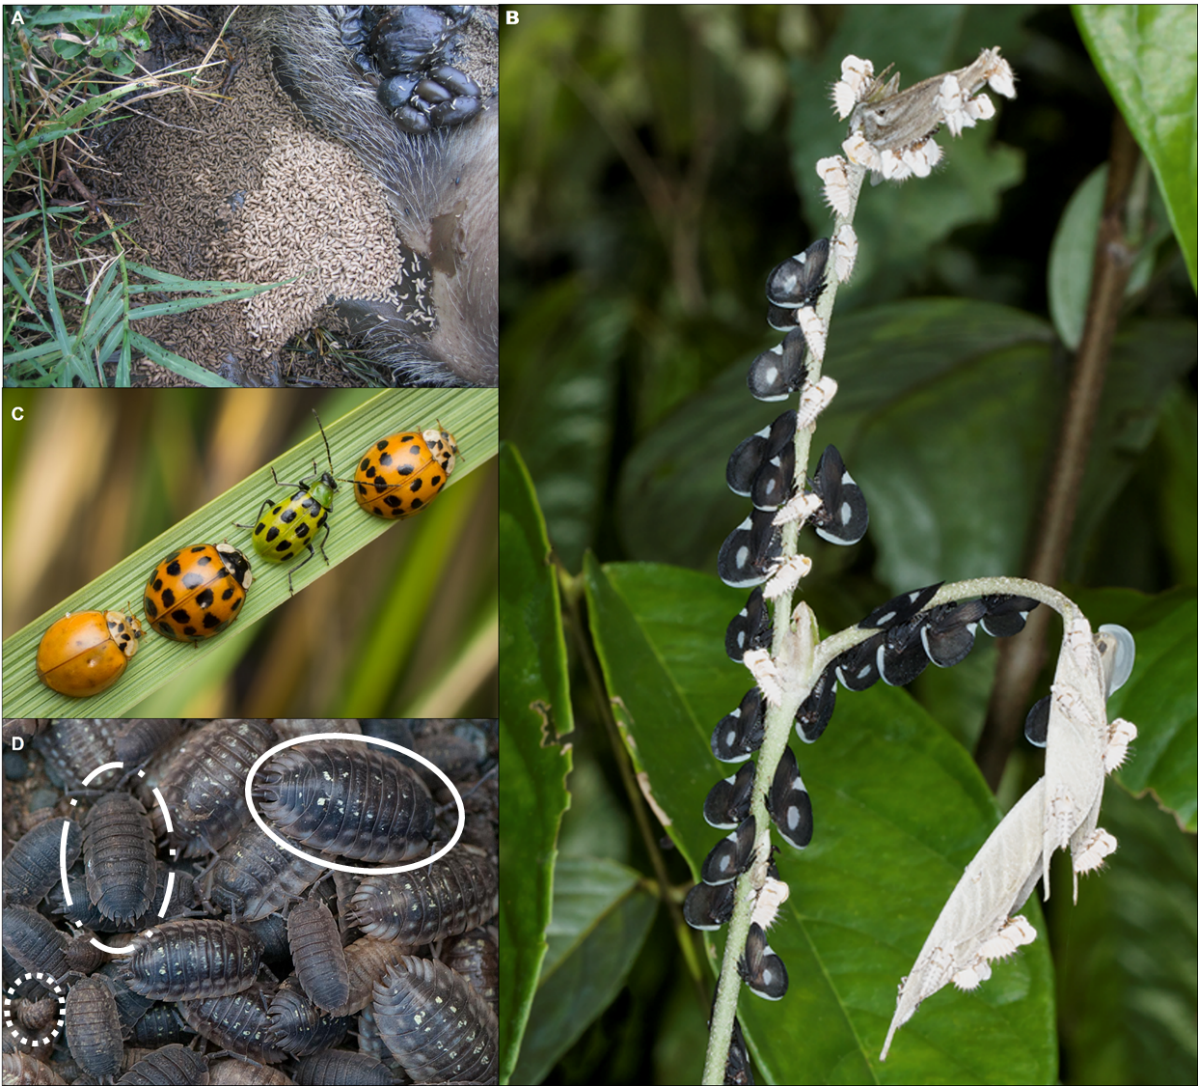
\includegraphics[width=0.9 \textwidth]{Figures/agreg_th_se.png}
		\rule{35em}{0.5pt}
	\caption[AgregMix]{\textbf{A.} Large mixed-species group of necrophagous Diptera larvae (\textit{Chrysomya albiceps} (dark maggots) and \textit{C. marginalis} (light maggots). Species segregation is observed due to the specific thermal preferences of the larvae (used with permission – Cameron Richards). \textbf{B.} Lady beetles (\textit{Harmonia axyridis}) and the spotted cucumber beetle (\textit{Diabrotica undecimpunctata}) on grass (used with permission - Nash Turley). \textbf{C.} Large mixed-species group of woodlice composed of three species (\textit{Armadillidium vulgare} (dotted circle), \textit{Oniscus asellus} (plain circle) and \textit{Porcelio scaber} (dashed and dotted circle); creative commons - Dave Ingram). \textbf{D.} A mixed-species group of treehoppers composed of adults and nymphs (white) of \textit{Membracis elevata} (black adults with a white spot on their back) and \textit{M. dorsata} (adults without a white spot) found in Ecuador (use with permission - Robert Oelman).}
	\label{fig:agregmix}

\end{figure}
    
%----------------------------------------------------------------------------------------
%	SECTION 4
%----------------------------------------------------------------------------------------
	\section{Benefits}
Aggregation is one of the mechanisms that can explain the coexistence of multiple species in patchy environments \cite{ives_aggregation_1991}. The advantages of mixed-species groups can be attributed to the increase in group size, which also occurs in non-mixed groups, and individuals cooperate to reach an optimal group size so that each individual will gain direct benefits. However, while it may seem that the benefits of grouping are more or less equally shared when individuals belong to the same species, this assumption becomes questionable for groups composed of different species. Surprisingly, even though mixed-species groups are interesting models to explore such questions, almost no experimental data can be found in the literature. Some examples of the benefits offered by mixed-species groups include protection against predators, protection against environmental constraints and foraging advantages resulting from aggregation behavior \citep{parrish_complexity_1999,riipi_multiple_2001,weed_benefits_2010}. 

		\subsection{Protection against predators}
One of the best studied benefits of aggregation is protection against predators, and this behavior is commonly believed to be one of the main advantages of aggregating in non-mixed and mixed-species groups \citep{evans_insect_1990,vulinec_collective_1990}. 
Cooperative defense, or the many eyes and ears theory, is one of the few benefits that have been studied in mixed-species groups. This advantage can be provided more efficiently in a mixed-species group than in a conspecific one because individuals of each species use their specific attributes to detect predators. For example, \textit{Panulirus guttatus} (a reef-obligate lobster) and \textit{P. argus} (a temporary reef-dwelling lobster) form mixed-species groups, and the two species are able to both perceive interspecific aggregation cues as well as each other’s alarm odors \cite{briones-fourzan_influence_2008}. These species share the same predators \cite{lozano-alvarez_coexistence_2007}, which can be better avoided by sharing alarm odors. 

		\subsection{Protection against the environment}
Aggregation by woodlice has been shown to offer protection against water loss (Figure \ref{fig:agregmix}; \cite{broly_effects_2014}). Woodlice are fully terrestrial crustaceans that are very sensitive to water loss, and \citet{hassall_effects_2005} demonstrated that two species of woodlice, \textit{Porcellio scaber} and \textit{Armadillidium vulgare}, clump together. These authors further found that at low densities, mixed-species groups promote population growth resulting in positive fitness consequences (higher growth rates and survivorship of group members; \cite{hassall_effects_2005}). Interestingly, \textit{A. vulgare} is more resistant to desiccation than \textit{P. scaber} \cite{hassall_effects_2005}, and \citet{broly_body_2015} subsequently demonstrated that body shape explains the difference in the mass-specific water loss rates between \textit{A. vulgare} and \textit{P. scaber}. Accordingly, \textit{P. scaber} aggregates more than \textit{A. vulgare} \cite{hassall_predicting_2010}, and it can be supposed that \textit{P. scaber} joins with \textit{A. vulgare} to form a larger group that is better able to withstand low relative humidity and/or high ambient temperatures. \citet{hassall_effects_2005} also hypothesized that this type of gathering offers members an additional food resource; woodlice are detritivorous and feed on each other’s feces.

		\subsection{Food assimilation}
Living together improves the assimilation of food in some mixed-species groups, and a good example is the larvae of carrion flies on a decaying cadaver (Figure \ref{fig:agregmix}; \cite{rivers_physiological_2011}). Maggot masses can contain hundreds to thousands of individuals from several species and instars, and the larvae secrete digestive enzymes (from their salivary glands) and mechanically liquefy muscles to facilitate the assimilation of food (exodigestion). This benefit is likely a consequence of a simple numerical effect; if more individuals are present in a group (regardless of the species), more salivary enzymes are produced \cite{wilson_impacts_2015}. \citet{dos_reis_larval_1999} observed a better survival rate in double-species groups composed of \textit{Chrysomya putoria} and \textit{Cochliomyia macellaria} when they increased the larval density of both species. They also showed that \textit{C. macellaria} is an inferior competitor in the presence of \textit{Ch. putoria}, so coexistence can occur. Obviously, such coexistence depends on the condition that the cadaver size is not limiting (competition phenomenon). \citet{ives_aggregation_1991} quantified the strength of larval competition in carrion flies and demonstrated a reduction in interspecific competition compared to intraspecific competition through resource partitioning.


%----------------------------------------------------------------------------------------
%	LE TABLEAU - DEBUT
%----------------------------------------------------------------------------------------
\begin{landscape}
\begin{table}
	\caption{Known examples of mixed-species groups in different arthropods’ taxons.\\ A: Artificial; F: Frequent; P: Punctual; R: Rare; $\uparrow$: increase; $\downarrow$: decrease; ???: unknown.}
	\label{tab:mixedsp}
	\centering
	\begin{tabular*}{\linewidth}{@{\extracolsep{\fill}}ccccccc}
		 \toprule
         \textbf{Taxons}				& \textbf{Species}		& \textbf{Life Stage}		& \textbf{Apparition}		& \textbf{Benefits}		&\textbf{Underlying}		&\textbf{References}\\
									&		&		&		&		& \textbf{Mechanisms}		&\\
		 \midrule
		\textbf{Ants}	& \textit{Manica rubida},		& Adults \& Juveniles		& A		&???		&???		&\citep{fielde_artificial_1903,errard_development_1994,vienne_congruency_1995}\\
        					& \textit{Formica selysi}	&	&	&	&	&\\	
            &	&	&	&	&	&\\                
        	& \textit{Azteca constructor},	& Adults \& Juveniles	&P	& $\uparrow$ Production of workers,	& Pleometrotic	&\citep{choe_evolution_1997,aron_les_2009}\\ 
            & \textit{A. xanthacrona}	&	&	&Better reproduction success	& (two queens)	&\\
            &	&	&	&	&	&\\
        
		\textbf{Aphids}	& \textit{Callipterinella calliptera},		& Adults \& Juveniles		& F		& $\uparrow$ Productivity of honeydew,	&Aggregation 	& \cite{hajek_coexistence_1986} \\
        & \textit{Betulaphis brevipilosa},	&	&	&Protection from predators	&pheromone?	& \\
        &	&	&	&	&	&\\

		\textbf{Butterflies}	& \textit{Malacosoma disstria},		& Adults \& Juveniles		&F		&Chemical protection,	&Trail-following 	&\citep{fitzgerald_specificity_1979,bogner_interspecific_1996}\\
        &\textit{M. americanum},	&	&	& Cannibalistic behavior	&abilities	&\\
        &\textit{Utetheisa sp}	&	&	&avoidance, Fitness (male	&	&\\
        &	&	&	&pheromone production)	&	&\\
        &	&	&	&	&	&\\
        
        \textbf{Carrion flies}	& \textit{Calliphoridae spp.},	&Adults \& Juveniles	&F	&Protection from 	&Shared  	&\citep{ives_aggregation_1991,dos_reis_larval_1999,woodcock_aggregation_2002,gunn_ability_2011,boulay_evidence_2013}\\
        &\textit{Sarcophagidae spp.},	&	&	&predators, Sharing 	&oviposition sites,	&\\
        &\textit{Muscidae spp.}	&	&	&salivary enzymes,	&Larval signal, 	&\\
        &	&	&	&Heat generation, &Thigmotactism,	&\\
        &	&	&	&$\uparrow$ Survival rate 	&Heat	&\\
        &	&	&	&	&	&\\
        
         \textbf{Cockroaches} &\textit{Nauphoeta cinera}, 	&Adults	&R	&???	&Chemical cues	&\cite{everaerts_changes_1997}\\
         &\textit{Leucophae maderae}	&	&	&	&	&\\
         &	&	&	&	&	&\\
         
         \textbf{Crabs} &\textit{Pagurus}	&Adults \& Juveniles	&???	&???	&???	&\cite{meadows_analysis_1973}\\
          & \textit{bernhardus},	&	&	&	&	&\\
          &\textit{P. prideauxi}	&	&	&	&	&\\
          &	&	&	&	&	&\\
          
		\end{tabular*}
\end{table}

\end{landscape}

\begin{landscape}
\begin{table}
	
	\label{tab:mixedsp2}
	\centering
	\begin{tabular*}{\linewidth}{@{\extracolsep{\fill}}ccccccc}
          \textbf{Crustaceans}	&\textit{Calappa calappa},	&Juveniles	&???	&Habitat selection	&Chemical cues,	&\cite{lecchini_ecological_2010}\\
          &\textit{Pachygrapsus}	&	&	&	&Visual cues	&\\
          &\textit{planifrons},	&	&	&	&	&\\
          &\textit{Lysiosquillina}	&	&	&	&	&\\
          &\textit{maculata},	&	&	&	&	&\\
          &\textit{L. sulcata},	&	&	&	&	&\\ 	
          &\textit{Raoulserenea sp.},	&	&	&	&	&\\ 
          &\textit{Stenopus hispidus},	&	&	&	&	&\\ 
          &\textit{Panulirus}	&	&	&	&	&\\ 
          &\textit{penicillatus}	&	&	&	&	&\\ 
          &	&	&	&	&	&\\
          &\textit{Panulirus guttatus},	&Adults	&R	&Recognition	&Chemical cues	&\citep{lozano-alvarez_coexistence_2007,lozano-alvarez_den_2001,briones-fourzan_influence_2008}\\ 
          &\textit{P. argus}	&	&	&alarm ordors,	&	&\\
          &	&	&	&Sharing shelter	&	&\\
          &	&	&	&	&	&\\
          
          \textbf{Fleas}	&40 species	&Adults \& Juveniles	&P	&Suppression of	&Reduction of the	&\citep{krasnov_aggregation_2006,krasnov_larval_2005}\\ 
          & listed by 	&	&	&host immune	&resource site	&\\
          &\citet{stanko_mammal_2002}	&	&	&	&	&\\
          &	&	&	&	&	&\\
          
          \textbf{Fruit flies}	&\textit{Drosophila sp.}	&Adults \& Juveniles	&F	&Limit fungal	&Chemical cues	&\citep{jaenike_aggregation_1991,wertheim_effects_2006,wertheim_evolutionary_2005}\\
          &	&	&	&	&Eggs-batches,	&\\
          &	&	&	&	&Non-random	&\\
          &	&	&	&	&distribution of	&\\
          &	&	&	&	&oviposition sites	&\\
          &	&	&	&	&	&\\
           
	\end{tabular*}
    \end{table}
		
\end{landscape}

\begin{landscape}
\begin{table}
	
	\label{tab:mixedsp3}
	\centering
	\begin{tabular*}{\linewidth}{@{\extracolsep{\fill}}ccccccc}
          \textbf{Lady beetles}	&\textit{Hippodamia}	&Adults	&P	& $\downarrow$ Mortality during	&Presence of	&\citep{simpson_aggregations_1975,lee_aggregation_1980,copp_temperature-dependent_1983,honek_aggregation_2007}\\ 
          &\textit{convergens, H.}	&	&	&winter, Protection 	&aphid prey,	&\\
          &\textit{tredecimpunctat},	&	&	&from predators	&Environmental	&\\
          &\textit{Hypera postica}	&	&	&and/or parasitoids?	&stimuli (T$\up{o}$, wind),	&\\
          &	&	&	&	&Chemical cues	&\\
          &	&	&	&	&	&\\
          
          \textbf{Locusts}	&\textit{Locusta migratoria}	&Juveniles	&F	&Protection from	&Chemical cues	&\citep{uvarov_grasshoppers_1977,niassy_intra-_1999}\\
          &\textit{migratorioides},	&	&	&predators	&	&\\
          &\textit{Schistocerca}	&	&	&	&	&\\
          &\textit{gregaria}	&	&	&	&	&\\
          &	&	&	&	&	&\\
          
          \textbf{Mites}	&\textit{Eotetranychus sp.},	&Juveniles	&F	&$\uparrow$ Fertility, 	&Deposition of	&\citep{slone_spatial_1999,le_goff_benefits_2011}\\
          &\textit{Tetranychus urticae}	&	&	&$\uparrow$ Silk production,	&faeces, Intraguild	&\\
          &	&	&	&$\uparrow$ Survival rate	&predation, Chemical	&\\
          &	&	&	&	&cues, Silk attraction	&\\
          &	&	&	&	&(sericophily)	&\\
          &	&	&	&	&	&\\
          
          \textbf{Scorpions}	&\textit{Buthotus judaicus},	&Adults	&P	&???	&Depends on season,	&\cite{warburg_intra-_2000}\\
          &\textit{Compsobuthus}	&	&	&	&Specialization of	&\\ 
          &\textit{werneri judaicus},	&	&	&	&scorpions for	&\\
          &\textit{Leiurus}	&	&	&	&different prey,	&\\
          &\textit{quinquestriatus}	&	&	&	&Low aggresiveness	&\\
          &	&	&	&	&	&\\
          
          \textbf{Spiders}	&\textit{Hypochilus thorelli},	&Adults \& Juveniles	&F	&Web-building,	&Chemical cues,	&\cite{hodge_conspecific_1997}\\
          &\textit{Achaearanea}	&	&	&Web-site selection	&Vibrational cues	&\\
          &\textit{tepidariorum}	&	&	&	&Silk attraction	&\\
          &	&	&	&	&(sericophily)	&\\
          &	&	&	&	&	&\\
       
    \end{tabular*}
    \end{table}
		
\end{landscape} 
          
\begin{landscape}
\begin{table}
	
	\label{tab:mixedsp4}
	\centering
	\begin{tabular*}{\linewidth}{@{\extracolsep{\fill}}ccccccc}          
     	\textbf{Stink bugs}	&\textit{Nezara viridula},	&Juveniles	&F	&Protection against	&Tactile cues,	&\citep{ishiwatari_studies_1976,fucarino_chemical_2004}\\ 
        &\textit{Chlorochroa ligata},	&	&	&dessication,	&Chemical cues	&\\
        &\textit{C. sayi, Thyanta}	&	&	&Developmental	&	&\\
        &\textit{pallidovirens},	&	&	&acceleration,	&	&\\
        &\textit{Euschistus}	&	&	&$\downarrow$ Mortality,	&	&\\
        &\textit{conspersus},	&	&	&$\downarrow$ Predation rates,	&	&\\
        &\textit{Eurydema sp.}	&	&	&Better adherence to	&	&\\
        &	&	&	&substrate	&	&\\
        &	&	&	&	&	&\\
     
     	\textbf{Termites}	&\textit{Reticulitermes}	&Adults \& Juveniles	&A	&???	&Chemical cues	&\cite{vauchot_regulation_1996}\\
        &\textit{santonensis},	&	&	&	&	&\\
        &\textit{R. lucifugus grassei}	&	&	&	&	&\\
        &	&	&	&	&	&\\
        
        \textbf{Thumbtack}	&\textit{Macrolophus}	&Adults	&P	&???	&???	&\cite{moreno-ripoll_conspecific_2012}\\
        &\textit{pygmaeus},	&	&	&	&	&\\
        &\textit{Nesidiocoris tenuis}	&	&	&	&	&\\
        &	&	&	&	&	&\\
        
        \textbf{Ticks}	&\textit{Haemaphysalis}	&Juveniles	&F	&$\downarrow$ Water loss	&Chemical cues	&\citep{sonenshine_pheromones_1985,tsunoda_interspecific_2007}\\
        &\textit{longicornis, H.}	&	&	&	&	&\\
        &\textit{megaspinosa}	&	&	&	&	&\\
        &	&	&	&	&	&\\
        
        \textbf{Treehoppers}	&\textit{Aconophora nitida},	&Juveniles	&F	&Protection from	&Stochastic phenomenon or	&\citep{olmstead_effect_1990,wood_diversity_1993}\\
        &\textit{A. mexicana}	&	&	&predators,	&Shared oviposition	&\\
        &	&	&	&Maternal care	&sites by females	&\\
        &	&	&	&	&	&\\
        
        \textbf{Trilobites}	&\textit{Ampyx, Asaphellus}	&Adults	&???	&???	&???	&\cite{rabano_linear_????}\\
        &	&	&	&	&	&\\      
             
    \end{tabular*}
    \end{table}
		
\end{landscape}     

\begin{landscape}
\begin{table}[t]
	
	\label{tab:mixedsp5}
	\centering
	\begin{tabular*}{\linewidth}{@{\extracolsep{\fill}}ccccccc}   
		\textbf{Whirligig beetles}	&\textit{Gyrinidae sp.}	&Adults	&F	&Predator avoidance,	&Mechanical stimuli	&\citep{heinrich_aggregation_1980,vulinec_aggregation_1989}\\
        &	&	&	&$\uparrow$ Defensive secretion	&(water waves),	&\\
        &	&	&	&	&Chemical cues	&\\
        &	&	&	&	&(pygidial secretion?),	&\\
        &	&	&	&	&Visual cues,	&\\
        &	&	&	&	&Orientation to	&\\
        &	&	&	&	&neighbours	&\\
        &	&	&	&	&	&\\
        
        \textbf{Woodlice}	&\textit{Porcelio scaber},	&Adults	&F	&Protection from	&Tactile cues,	&\cite{hassall_effects_2005}\\
        &\textit{Armadillidium vulgare},	&	&	&dessication,	&Chemical cues	&\\
        &\textit{Oniscus asellus}	&	&	&$\uparrow$ Production of faeces	&	&\\
        &	&	&	&(secondary food source)	&	&\\
        &	&	&	&	&	&\\
		\bottomrule
    \end{tabular*}
    \end{table}
		
\end{landscape}
 \clearpage
%----------------------------------------------------------------------------------------
%	LE TABLEAU - FIN
%----------------------------------------------------------------------------------------

%----------------------------------------------------------------------------------------
%	SECTION 5
%----------------------------------------------------------------------------------------
	\section{Species competition}
The close proximity of competitors that occupy the same ecological niche decreases food availability or the accessibility of reproductive partners, so competition can emerge between members of mixed-species groups in habitats with insufficient food resources. Indeed, even if aggregation offers advantages, there may also be unbalanced relationships or even social parasitism in mixed-species groups, which will engage the competitive abilities of each species. Moreover, mechanical exclusion of one species by another may also be observed. At first, individuals of one species cooperate with those of another to form a group, but once the group is formed and stable, species can mutually separate if their optimal group size is reached. If the two species have sufficiently different ecological niches, they can segregate but remain in contact (Figure \ref{fig:agregmix}; \cite{villet_contemporary_2010}), and it would be interesting to follow the dynamic of an aggregation at the moment when a group splits.

\citet{kuno_aggregation_1988} modified \textit{Volterra’s competition model} \cite{volterra_fluctuations_1926} and the generalized logistic function by incorporating \textit{Lloyd’s indices} of intra- and interspecific mean crowding \cite{lloyd_`mean_1967}. These upgraded models explain why some allied species coexist on the same resource patch, and \citet{kuno_aggregation_1988}) showed that \textit{(1) any increase in the patchiness of distribution facilitates intraspecific competition resulting in marked lowering of the equilibrium density for individual populations; but (2) its effect on the interspecific competition is just the opposite, relaxing the interaction and enabling different species sharing the same niche, which would otherwise be incompatible, to coexist stably.} Such models have been used to study competition exclusion in many species, but to our knowledge, these species did not form mixed groups.

In social foraging groups, \textit{the producer-scrounger game} is one of mathematical models used to describe the individual foraging strategies of group members \cite{giraldeau_social_2000}. This model highlights the exploitation of a producer’s findings (e.g., resource sites) by scroungers and predicts how foraging strategies change with food patch size. It also predicts how individuals can switch between the two strategies, scrounging or producing, until they reach an evolutionary stable strategy \cite{giraldeau_food_1999}. Such models have been used for many bird species \citep{giraldeau_social_2000,sumpter_collective_2009}, but to our knowledge, only in non-mixed species groups. This model could be modified to describe the foraging strategies of mixed-species groups by adding parameters to quantify the foraging abilities of each species. Such an upgraded model would be useful for predicting the ways in which species search and compete for resources in mixed groups.


%----------------------------------------------------------------------------------------
%	SECTION 6
%----------------------------------------------------------------------------------------
	\section{Metrics}
Different authors have used specific coefficients to study and quantify mixed-species groups. For this purpose, \citet{ives_aggregation_1991} proposed the quantity $\text{C}_{\text{A,B}}$ to measure mixed-species aggregations in carrion flies. 

\begin{equation}
	\label{equation1}
		C_{A,B}= \frac{Cov_{A,B}}{N_{A}N_{B}}  
\end{equation}

where $\text{Cov}_{\text{A,B}}$ is the covariance between species A and species B, and $\text{N}_{\text{A}}$ and $\text{N}_{\text{B}}$ are the number of ovipositing females on the same carcass or the number of emergent species A and B from individual breeding sites \cite{jaenike_aggregation_1991}. A value of 0.5 means a 50$\%$ increase in the expected number of heterospecific competitors in the same patch (i.e., if species A and species B are distributed independently) \cite{ives_aggregation_1991}. Using this parameter, Ives showed that aggregation behavior plays a major role in the coexistence of carrion fly species; he observed a 57$\%$ reduction in the average larval competition among pairs of species.
\citet{everaerts_changes_1997} used a \textit{cohabitation-coefficient} (CC) in their study of cockroaches (binary choice test between 2 resting sites):

\begin{equation}
	\label{equation2}
		CC= \frac{\sum n_{A}n_{B}}{10(N_{A}N_{B})}  
\end{equation}

where $\text{n}_{\text{A}}$ and $\text{n}_{\text{B}}$ are the respective numbers of species A and B under each shelter, and $\text{N}_{\text{A}}$ and $\text{N}_{\text{B}}$ are the total number of individuals of species A and B, respectively. A value of zero for CC indicates interspecific avoidance; a value of 0.33 represents a random distribution, and values higher than 0.33 indicate true interspecific aggregative behavior. An interesting feature of this relationship is that this coefficient can distinguish between avoidance of gregariousness and tolerance as the limit between these two behaviors (Figure \ref{fig:ever}). However, this method of quantifying mixed-species aggregations is restricted to experiments with two aggregation sites and is thus not useable under most field conditions.

 \begin{figure}[ht]
	\centering
		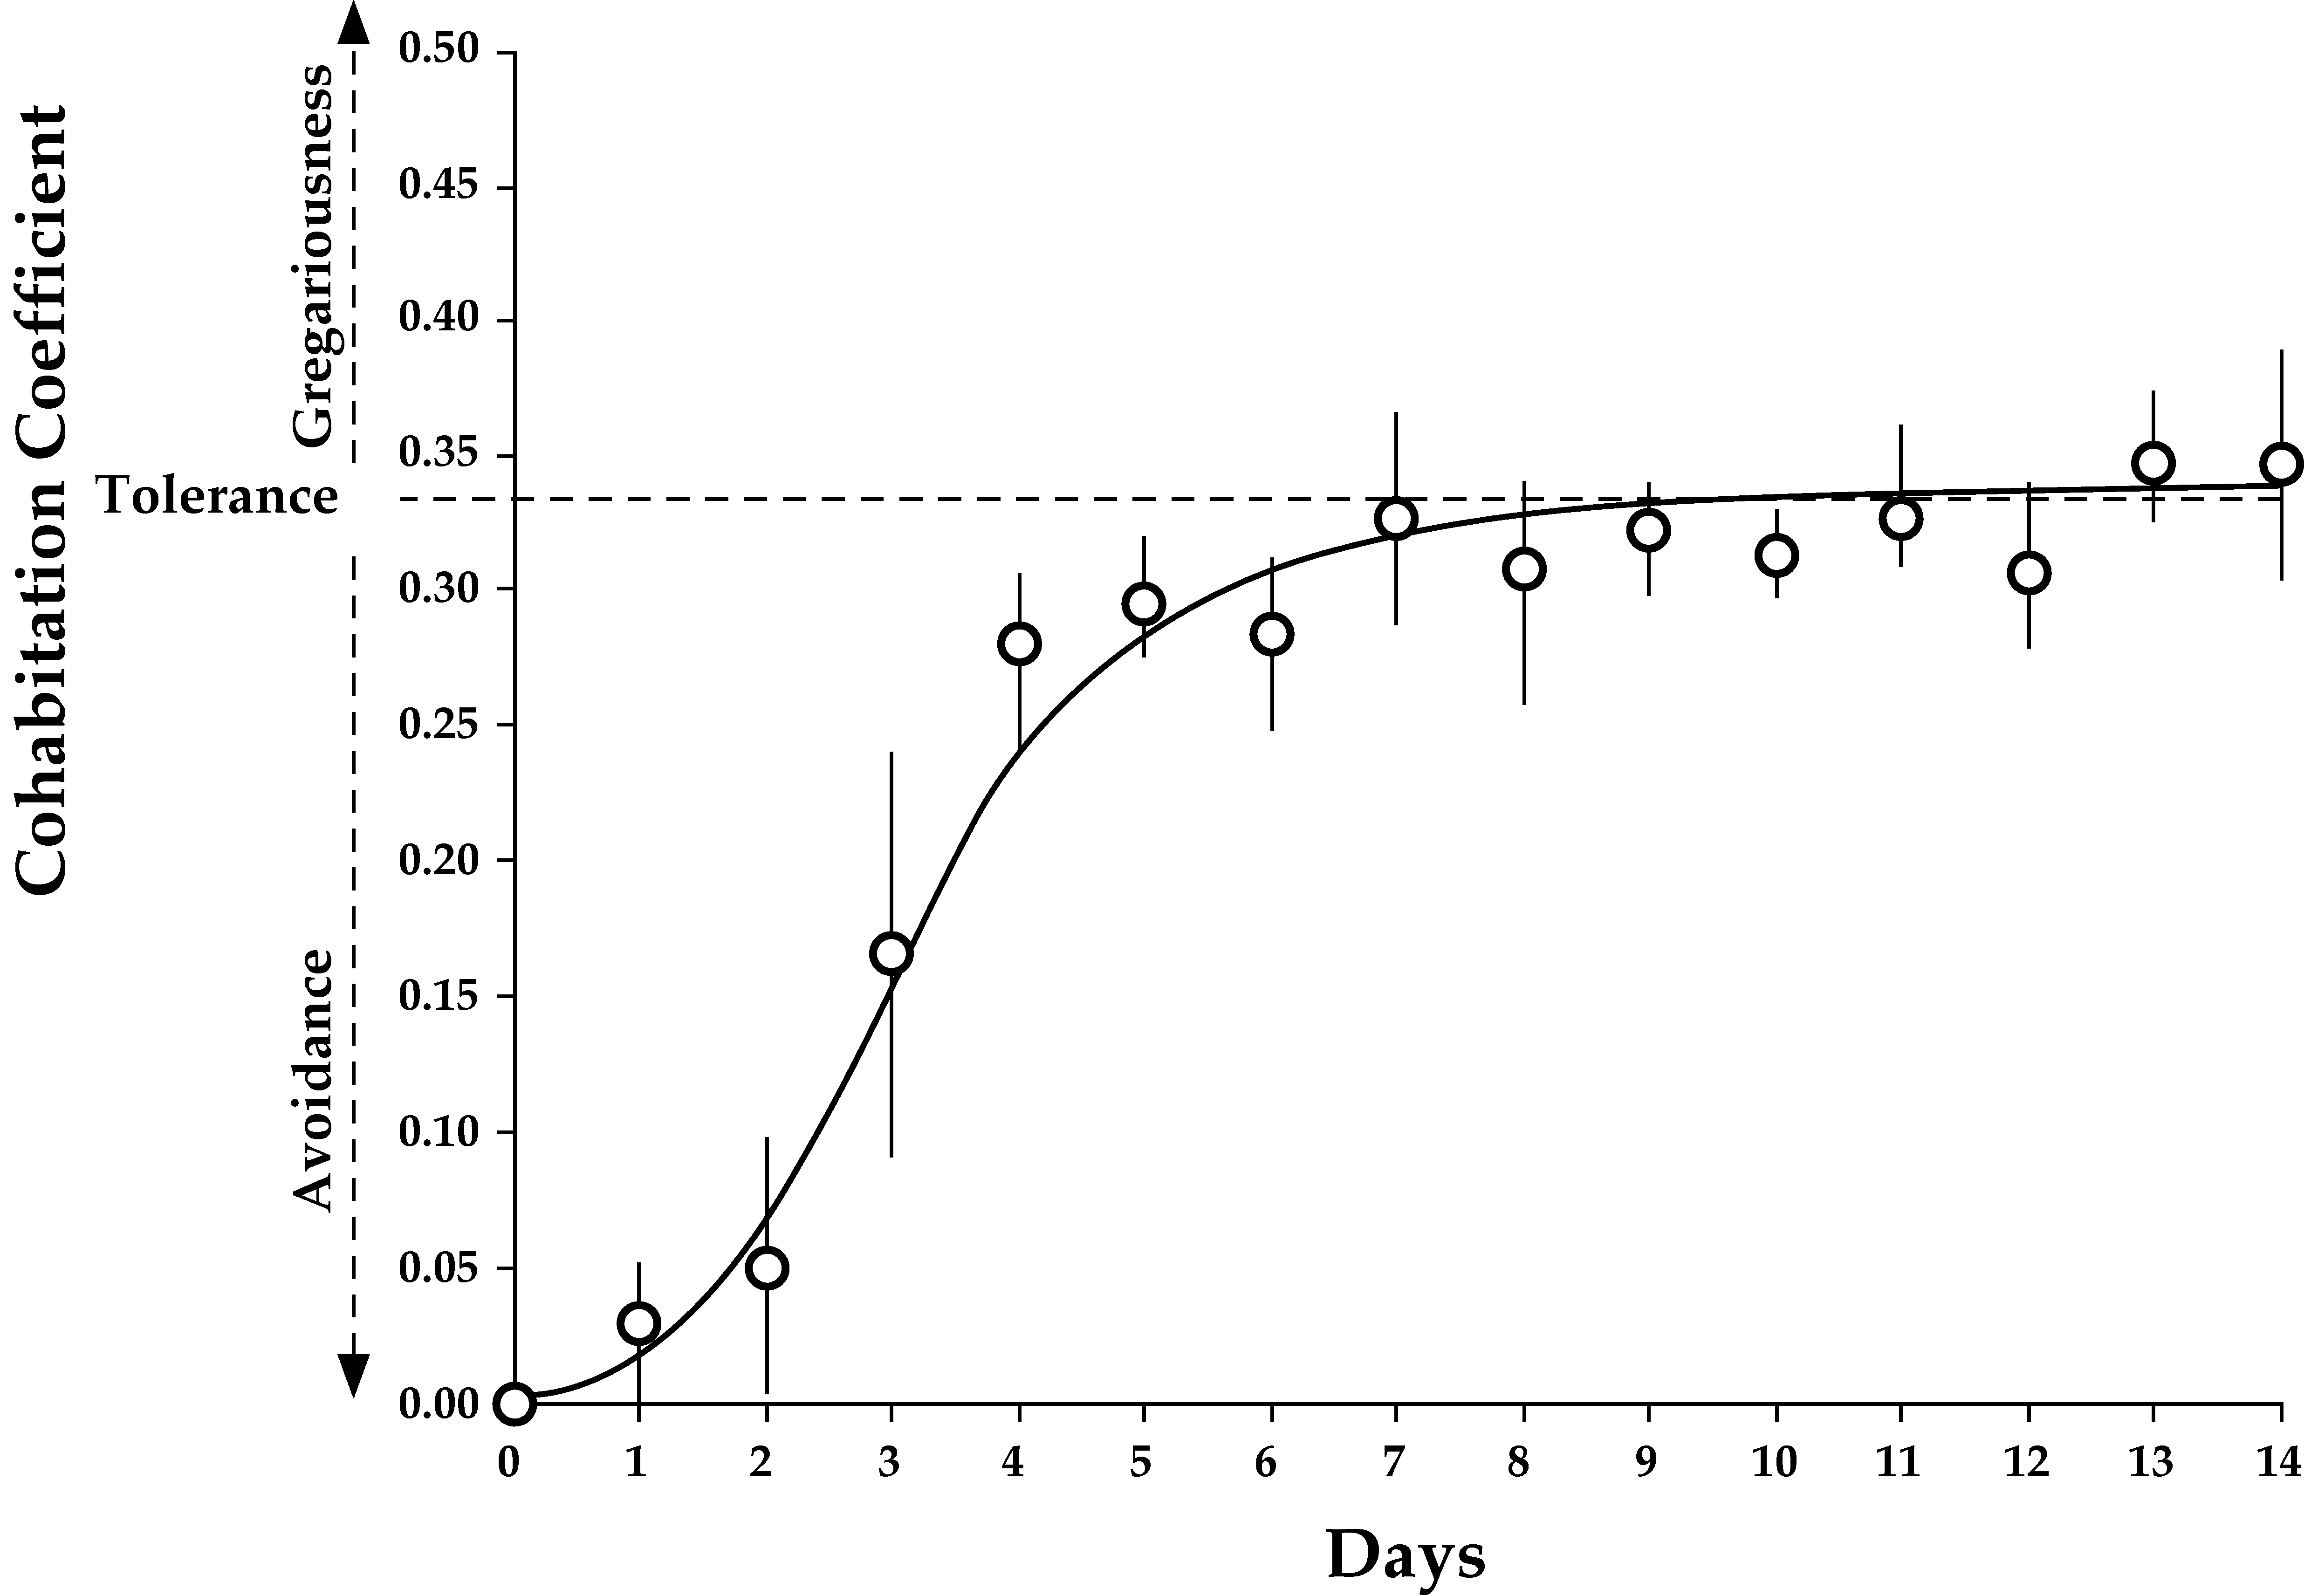
\includegraphics[width=0.9 \textwidth]{Figures/everaert_these.png}
		\rule{35em}{0.5pt}
	\caption[Ever]{The daily evolution of the \textit{cohabitation coefficient} (mean and range; equation \ref{equation2}) when two cockroach species (\textit{Nauphoeta cinerea} and \textit{Leucophaea maderae}) were maintained in heterospecific colonies (used with the permission of C. Everaerts).}
	\label{fig:ever}

\end{figure}

\citet{veech_intraspecific_2003} modified the coefficient C of \citet{ives_aggregation_1991} to measure the tendency for individuals of a species to aggregate with the individuals of other species (i.e., beetles and butterflies):

\begin{equation}
	\label{equation3}
		C= \left\lbrace\ \frac{\sum x_{i}h_{j}}{XN} - H \right\rbrace	\frac{1}{H}  
\end{equation}

where $\text{x}_{\text{j}}$ is the number of individuals at site j; X is the mean number of individuals per site; N is the number of sites; $\text{h}_{\text{j}}$ is the number of heterospecific individuals at site j; and H is the mean of all of the sites. A positive increase in C indicates an increase in the mixed-species aggregation, whereas an increasingly negative value represents interspecific repulsion. In their study, \citet{veech_intraspecific_2003} clearly showed that intraspecific aggregation decreases local species diversity, but interspecific aggregation promotes it.



%----------------------------------------------------------------------------------------
%	SECTION 6
%----------------------------------------------------------------------------------------
	\section{Examples}
Some mixed-species aggregations have been reported in arthropods, from aphids to butterflies and woodlice to ants (Figure \ref{fig:agregmix}, Table \ref{tab:mixedsp}; \cite{costa_other_2006}), and they have been observed in terrestrial, aquatic and flying arthropods (Table \ref{tab:mixedsp}). These groups can be composed of juveniles, adults or, in the majority of cases, both stages. We have listed four categories of mixed-species aggregations: frequent (F), punctual (P), rare (R) and artificial (A) (Table \ref{tab:mixedsp}). 

A frequently reported example is the mixed-species aggregation of nymph and adult treehoppers, or \textit{Aconophora species} (Figures \ref{fig:agregmix} and \ref{fig:acono}), but this aggregation involves both the mixed-species aggregation of the nymphs and a mutualism with ants. \cite{wood_diversity_1993} hypothesized that this type of mixed-species aggregation could result from transport by ants, and indeed, the ants collect sugar secreted from the nymphs and protect them from predators. Female treehoppers also aggregate their eggs in response to resource limitation (food or oviposition sites; \cite{wood_sociality_1979}), but ant attacks can occur if the nymph aggregations are disturbed by the rapid movement of adult treehoppers \cite{wood_diversity_1993}. In such cases, aggregation is supposed to allow for more efficient communication among treehopper females to prevent the attacks. Depending on the context, this mixed-species interaction can turn into either cooperation \cite{olmstead_effect_1990} or conflict \cite{wood_diversity_1993}.

 \begin{figure}[ht]
	\centering
		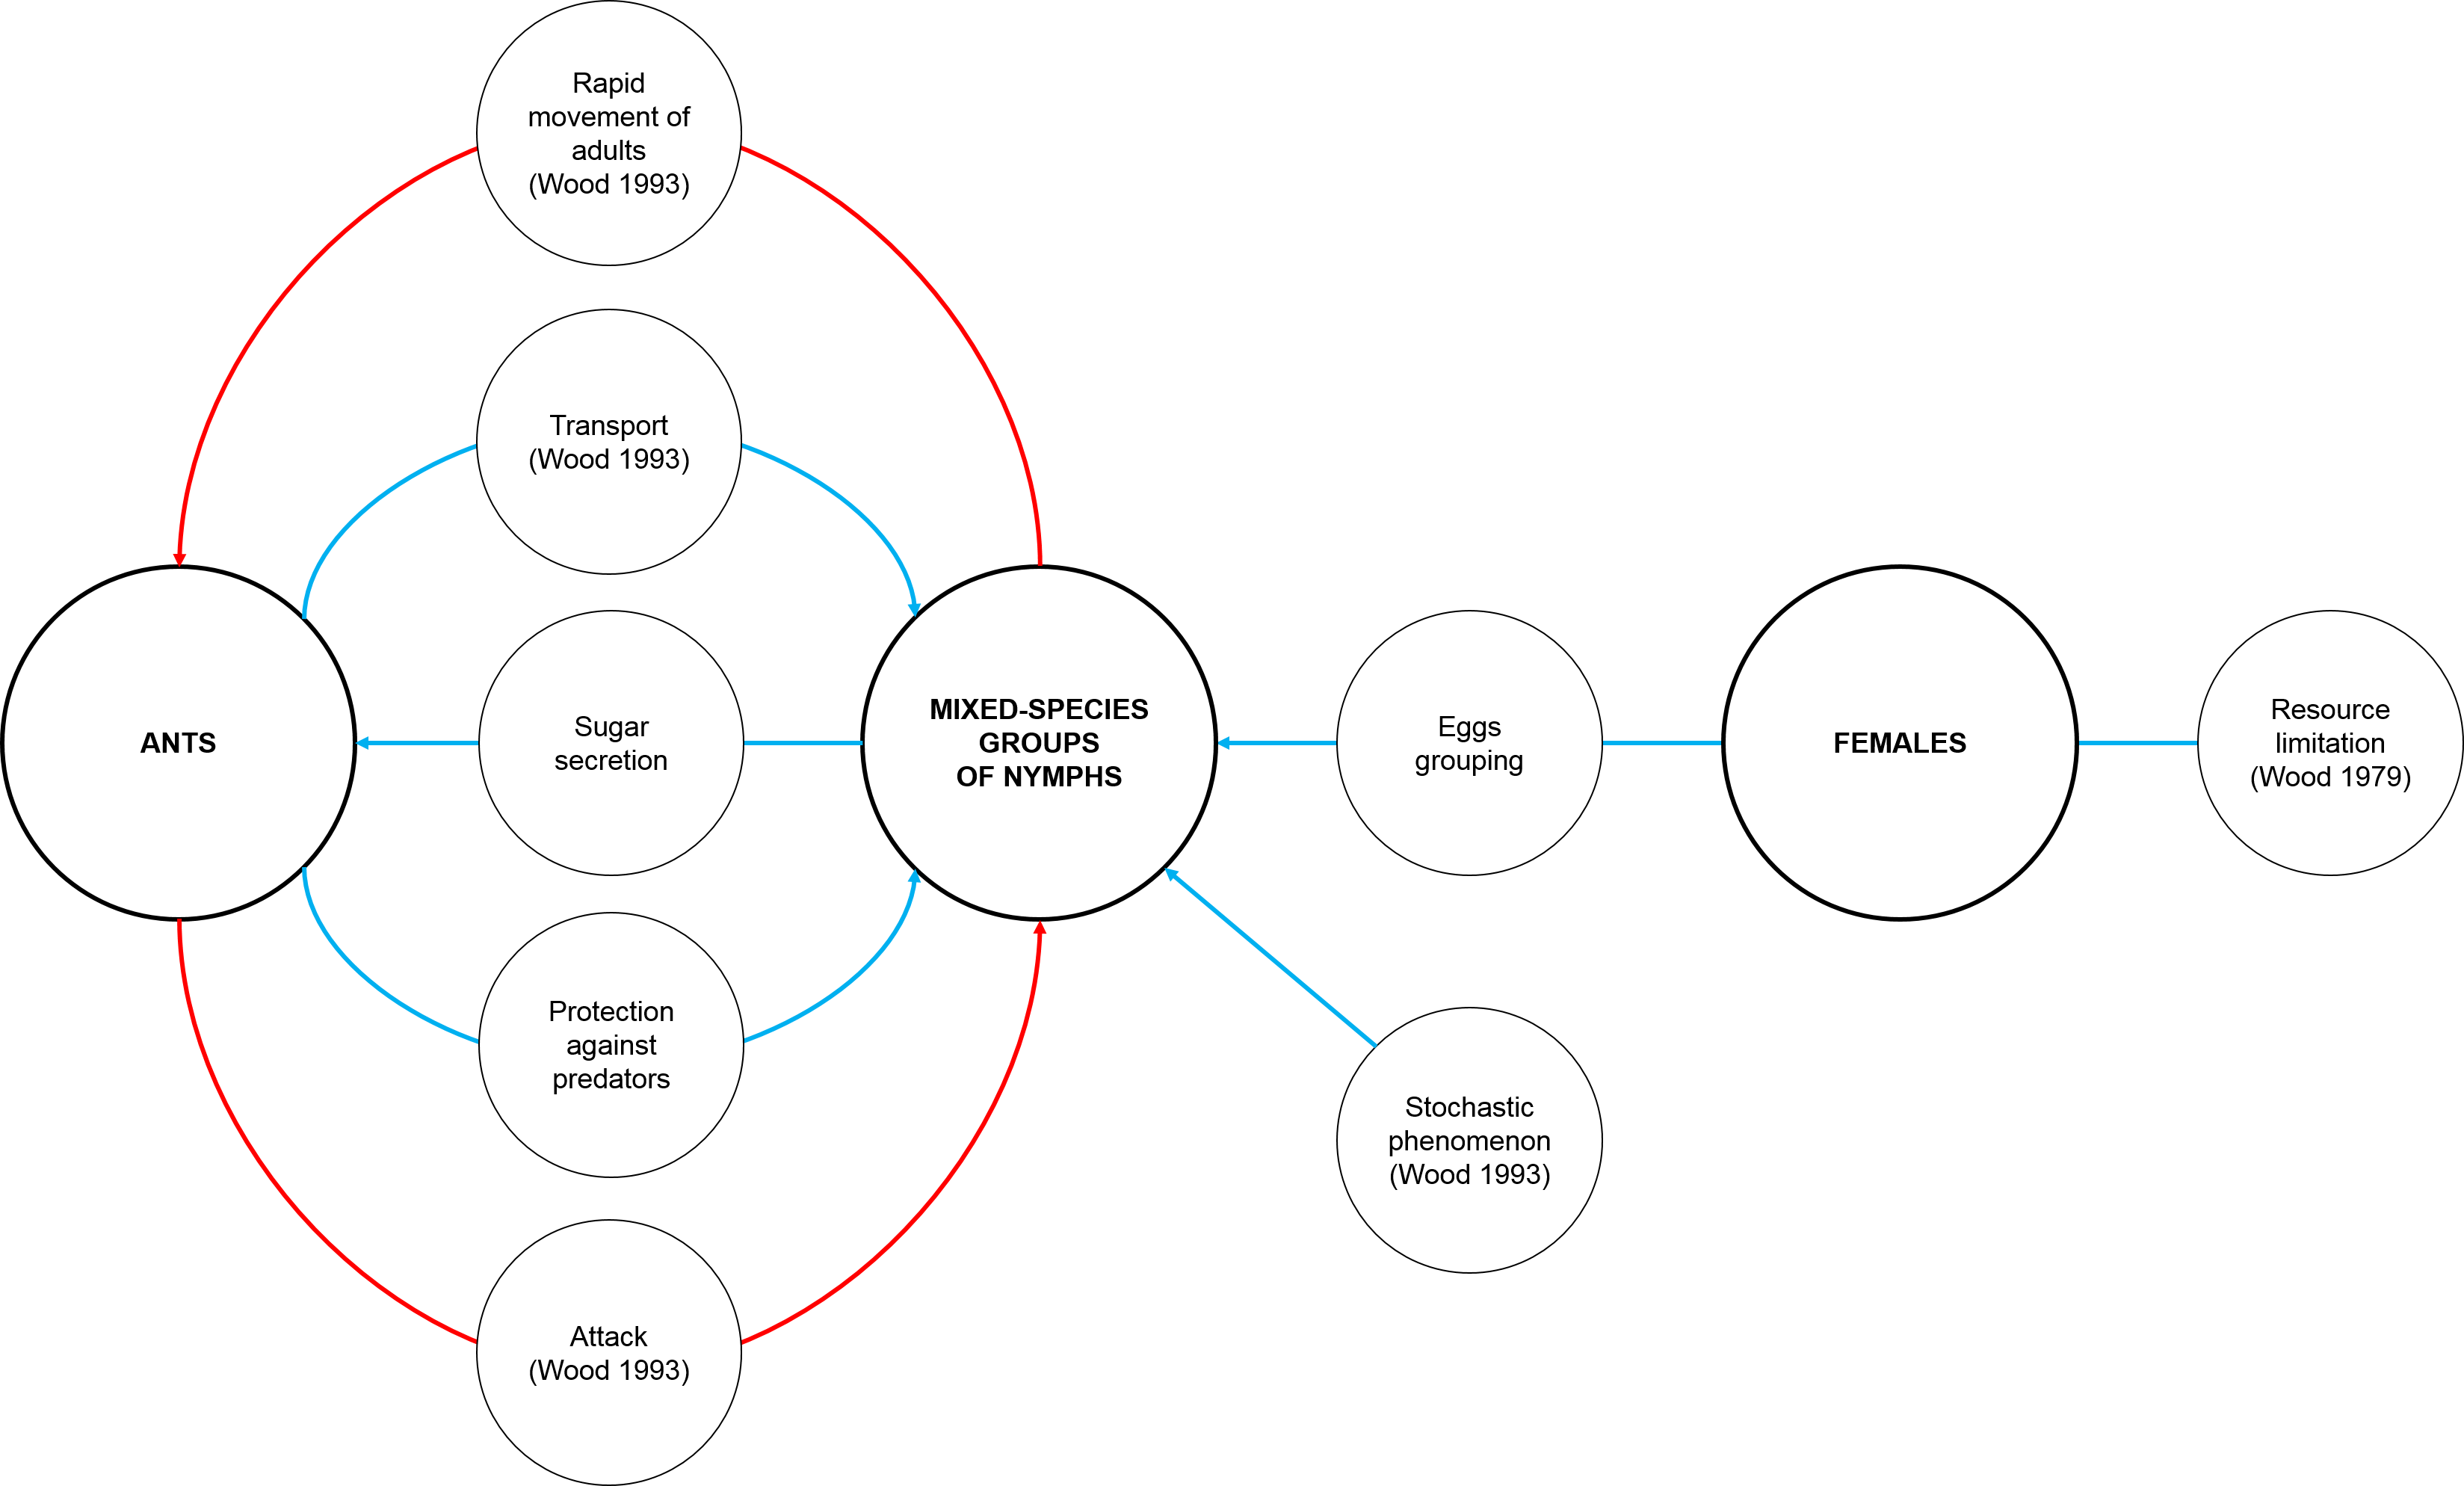
\includegraphics[width=0.9 \textwidth]{Figures/acono.png}
		\rule{35em}{0.5pt}
	\caption[Acono]{ Schematic overview of the mechanisms underlying mixed-species groups in treehoppers. Blue lines correspond to positive feedbacks that promote the formation of mixed-species groups, and red lines indicate negative feedbacks (based on Wood \citep{wood_sociality_1979,wood_diversity_1993}).}
	\label{fig:acono}

\end{figure}

Punctual mixed-species groups often appear at a given time each year. Ladybeetles, or ladybugs, form large, mixed-species aggregations inside buildings during winter \citep{simpson_aggregations_1975,lee_aggregation_1980}, and by forming such groups, ladybeetles can conserve heat and reduce their mortality due to cold \cite{copp_temperature-dependent_1983}. \citet{durieux_role_2012} highlighted the role of cuticular hydrocarbons in non-mixed Harmonia axyridis groups and identified chemical compounds, principally saturated hydrocarbons, with the capacity for heat retention on individuals \cite{durieux_role_2012}. It could be interesting to perform behavioral tests on mixed-species groups to observe the possible interspecific recognition of these hydrocarbons. Such experiments have not been performed, but they could provide interesting information about inter-specific recognition mechanisms in mixed-species groups. 

Mixed-species groups have also been observed in some lobster species, such as \textit{Panulirus guttatus} and \textit{P. argus} \citep{lozano-alvarez_coexistence_2007,briones-fourzan_influence_2008} (Table \ref{tab:mixedsp}). This type of gathering forms due to stochastic phenomena (by chance) rather the intention of individuals to aggregate \cite{briones-fourzan_influence_2008}. \textit{Panulirus guttatus} and \textit{P. argus} randomly share the same shelters \cite{lozano-alvarez_coexistence_2007}; the former tends to cling to the walls while the latter occupies the floor. \citet{briones-fourzan_influence_2008} suggested that such rarely observed mixed-species groups could be chemically mediated. Each species uses the shelter space differently, which promotes coexistence, and the aggregation allows \textit{P. argus} to share the alarm odors of \textit{P. guttatus}, enhancing protection against predators. The mechanisms underlying the avoidance behavior of \textit{P. argus} to the alarm odors of \textit{P. guttatus} remain unknown. However, \citet{briones-fourzan_influence_2008} supposed that the sedentary and defensive behavior of \textit{P. guttatus} (to go deeply into the shelter) could be sufficiently adaptive to avoid the need to recognize the alarm odors of \textit{P. argus}.

Lastly, some artificial groups have been observed but only under laboratory conditions and often in highly social species, such as ants or termites (Table \ref{tab:mixedsp}). In 1994, Errard \cite{errard_development_1994} reared \textit{Manica rubida} and \textit{Formica selysi}, two ant species, in a mixed-species colony during different time periods and observed a gradual increase in the tolerance behavior of both species over time. Furthermore, the individual hydrocarbon profiles of both species gradually acquired the chemical profile of the mixed colony \cite{errard_development_1994}. The establishment of the social group occurred in the early adult stage and was maintained through the imprint of mixed-colony cuticular hydrocarbons (imprinting-like phenomena). Interestingly, the individuals reared in the mixed-species colony were not attacked by allospecific individuals reared with non-mixed nestmates, suggesting that there is a minimal quantity of allospecific hydrocarbon compounds necessary for allospecific recognition \cite{errard_development_1994}. Such observations support the fact that mixed-species groups are composed of phylogenetically related species, which has been verified by the examples listed in Table \ref{tab:mixedsp}. Phylogenetic proximity likely facilitates cross-species recognition, a mechanisms needed to initiate and maintain mixed-species groups. Aggregates are less likely to be formed by species that relatively different phylogenetically, e.g., the ant and treehopper relationship (Figure \ref{fig:acono}; \cite{wood_sociality_1979}); the term mutualism is used to characterize such interspecific interactions. 

    
%----------------------------------------------------------------------------------------
%	SECTION 7
%----------------------------------------------------------------------------------------
	\section{Cross-species recognition}    
To create groups, animals use their ability to recognize and remain with conspecifics. Kin recognition has been well documented in several arthropod species \citep{wilson_kin_2005,costa_other_2006,jeanson_conspecific_2007,lihoreau_kin_2007,lihoreau_kin_2009,lize_kin_2010}. This recognition is mostly based on the perception of chemical cues (e.g., cuticular hydrocarbons) \citep{bell_searching_1990,chapman_insects:_1998}, and once aggregated, individuals must share information to stabilize, shape, reassemble or even split the group \cite{lachmann_advantages_2000}. This can be achieved using a range of vectors including chemical signals as well as visual recognition, and such vectors can also be used by individuals for cross-species recognition. These mechanisms imply that the aggregation vectors involved in intraspecific groups are alike, such as the similar chemical profiles of aggregation pheromones. 

		\subsection{Chemical recognition}
\citet{wertheim_evolutionary_2005} highlighted three types of interspecific interactions that are influenced by aggregation pheromones in Diptera and beetle species. The first is that aggregation pheromones are associated with microorganisms (bacteria or fungi). On plants or fruits, microbial infestation is directly associated with feeding by insects; microorganisms facilitate attack because healthy plants cannot be penetrated by larvae. For example, drosophilid females preferentially lay their eggs on host plants that have already been infested. Aggregation pheromones can also be associated with natural enemies; parasitoids that target Diptera can respond to the aggregation pheromones of their hosts \cite{wertheim_evolutionary_2005}. Lastly, aggregation pheromones can be associated with community ecology. \citet{wertheim_evolutionary_2005} described examples of cross-attraction in bark beetles. The composition of the aggregation pheromones of closely related species are similar, and this chemical similarity promotes mixed-species groups.

Another well-known example of sharing information in mixed-species groups is cockroaches. \citet{everaerts_changes_1997} reared two species of cockroaches together, namely, \textit{Nauphoeta cinera} and \textit{Leucophae maderae}, in the same environment. Far from expressing simple tolerance behavior (Figure \ref{fig:ever}), the individuals aggregated together, increasing the size of the group \cite{everaerts_changes_1997}. The authors also observed a change in the chemical profile of the hydrocarbons in both species. Under natural conditions, these chemical profiles are highly species-specific and used by cockroach species to aggregate \cite{lihoreau_kin_2009}, but when reared together, these two species established interspecific chemical communication. \citet{everaerts_changes_1997} hypothesized that this hydrocarbon transfer occurred during the frequent physical contact among group members. Such processes require relative phylogenetic proximity among species, and moreover, species likely need to be in long, cumulative physical contact to allow for chemical transfer. This contact occurs in the early life stages of individuals and persists over time. 

		\subsection{Visual recognition}
\citet{mizell_iii_congener_2012} described evidence of visual responses to conspecific and heterospecific congeners in two leafhopper species, \textit{Homalodisca vitripennis} and \textit{Oncometopia nigricans}. The authors used visual baits, such as leafhopper cadavers or colored models, to attract individuals, and the presence of conspecifics or heterospecific congeners was used to estimate the quality of the host plant. Using this information, leafhoppers chose to rejoin the heterospecific congeners or not. Similarly, \citet{lecchini_ecological_2010} showed that postlarval crustaceans preferentially used visual cues over chemical cues to detect heterospecific individuals and thus select their habitat. The presence of heterospecific crustacean congeners informs individuals about habitat quality and promotes mixed-species aggregation.


%----------------------------------------------------------------------------------------
%	SECTION 8
%----------------------------------------------------------------------------------------
	\section{Conclusion}  
Based on this review of the literature on mixed-species groups, mixed-species aggregations are found in a wide range of arthropod taxa (Table \ref{tab:mixedsp}). Such groups are not restricted by the degree of sociality of the species; they were observed in species ranging from presocial to eusocial. However, mixed-species grouping is restricted to species that live together or at least have the same habits. In other words, species that form stable social groups are more likely to accept individuals from other species, but mixed-species groups are usually composed of phylogenetically related species. This is likely due to the cross-species recognition process, which is essential for initiation and maintenance of a group. Closely related species are likely to share similar aggregation vectors (e.g., related chemical compounds), which facilitates their detection by heterospecific individuals and thus the formation of mixed-species groups. Chemical compounds are the most common aggregation cues used by arthropods in nature, and this communication can be olfactive, as in bark beetles \cite{wertheim_evolutionary_2005}, or tactile, as in cockroaches \cite{everaerts_changes_1997}. The study of cross-species detection of chemical signals is an interesting starting point to understand the mechanisms driving mixed-species aggregation, especially in the context self-organization. 

Compared to mixed-species groups, our understanding of intraspecific groups is more comprehensive (see the review by \citet{jeanson_key_2012}). Many of the experimental designs used to study monospecific groups, such as the binary choice test used by Leoncini and Rivault \cite{leoncini_could_2005}, can be applied to mixed-species groups of arthropods. Several marking techniques also exist to follow individuals, facilitating monitoring during experiments \cite{hagler_methods_2001}. Such experimental backgrounds provide a good working basis for further experimentation on mixed-species groups. Moreover, mathematical models have been developed to quantify mixed-species groups, but to our knowledge, models of the cooperation-competition phenomenon need to be established for mixed-species groups.

Mixed-species groups of arthropods provide similar benefits to members as intraspecific groups as well as those observed in mixed-species groups of mammals \cite{stensland_mixed_2003}. These benefits essentially include enhancing protection against predators and shared foraging strategies (Table \ref{tab:mixedsp}). Mixed-species groups can be stable, and the benefits can be shared among species if they do not have the same ecological niche or if resources are not limiting. However, interspecific competition can quickly turn the benefits toward one species at the expense of the other.

%----------------------------------------------------------------------------------------
%	SECTION 9
%----------------------------------------------------------------------------------------
	\section{Acknowledgments}  
Authors would like to thanks Claude \textsc{Everaerts} (Univ. Bourgogne), Robert \textsc{Oelman} (Photographer), Cameron \textsc{Richards} (PhD) and Nash \textsc{Turley} (Post-Doc) for giving us the permission of reuse their figure or photos.


\clearpage
    
    
        
    
    
    
    



